\chapter{Work Plan}
\lhead{\emph{Work Plan}}

\begin{figure}[h!]
  \centering
  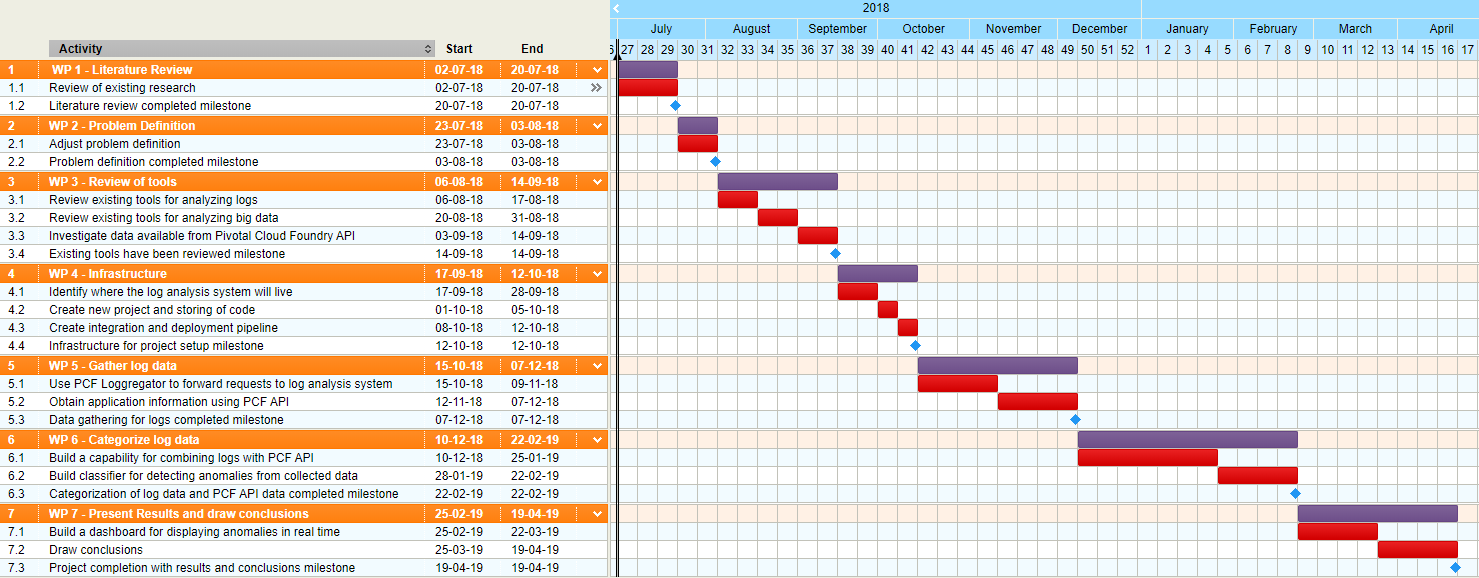
\includegraphics[width=1.0\textwidth]{./figures/gantt.png}
  \caption{gantt}
  \label{fig:gantt}
\end{figure}

\begin{itemize}
  \item \textbf{WP 1} Literature review - 3 weeks - In this work package a literature review on existing approaches to log analysis will be performed.
  
  \item \textbf{WP 2} Problem definition - 2 weeks - Based on the literature review, the challenges of log analysis will be evaluated further. The challenges will produce the definition of key research questions.
  
  \item \textbf{WP 3} Review of tools - 6 weeks - In this work package, available tools for log analysis will be looked at. Additionally, data available in the Pivotal Cloud Foundry API will be investigated.
  
\item \textbf{WP 4} Infrastructure - 4 weeks - This work package involves setting up the infrastructure for the project. Components such as code storage and continuous integration will be acquired and configured in order to enable rapid development. 
  
  \item \textbf{WP 5} Gather log data - 8 weeks - In this work package I will be sourcing logs that will be used for comparative analysis of my service. I will also be setting up Cloud Foundries loggregator to forward all logs to the analysis service.
  
  \item \textbf{WP 5} Gather log data - 8 weeks - This work package involves sourcing logs that will be used for comparative analysis of my service. Furthermore, setting up Cloud Foundry's Loggregator to forward all logs to the analysis service will be configured.
  
  \item \textbf{WP 6} Categorize log data - 11 weeks - In this work package the delivery of the necessary log analysis algorithms to correctly identify root causes of failures will be performed. A comparison of the benefits of using log analysis with and without PCF API information will be done.
    
  \item \textbf{WP 7} Present Results and draw conclusions - 8 weeks - This work package will deliver a dashboard to display root causes of issues to users. Once complete a report outlining the project observations and conclusions will be written.
\end{itemize}

The milestones that are set to be achieved through the above work packages are as follows.

\begin{enumerate}
  \item Literature review completed
  \item Problem definition completed
  \item Existing tools have been reviewed 
  \item Infrastructure for project setup 
  \item Data gathering for logs completed
  \item Categorization of log data and PCF API data completed
  \item Project completion with results and conclusions
\end{enumerate}